\subsection{Cook membrane problem}

The cook membrane problem \cite{simo1990} is used herein for stability analysis of pressure. The geometry of this problem is shown in Figure \ref{fg:cook_illsutration},
in which the left hand side is fixed and the right hand side subjects a concentrated force $P=1000$ in $y$--direction.
The material parameters are Young's modulus $E=3\times 10^6$ and Poisson's ratio $\nu=0.5-10^{-8}$.

\begin{figure}[H]
\centering
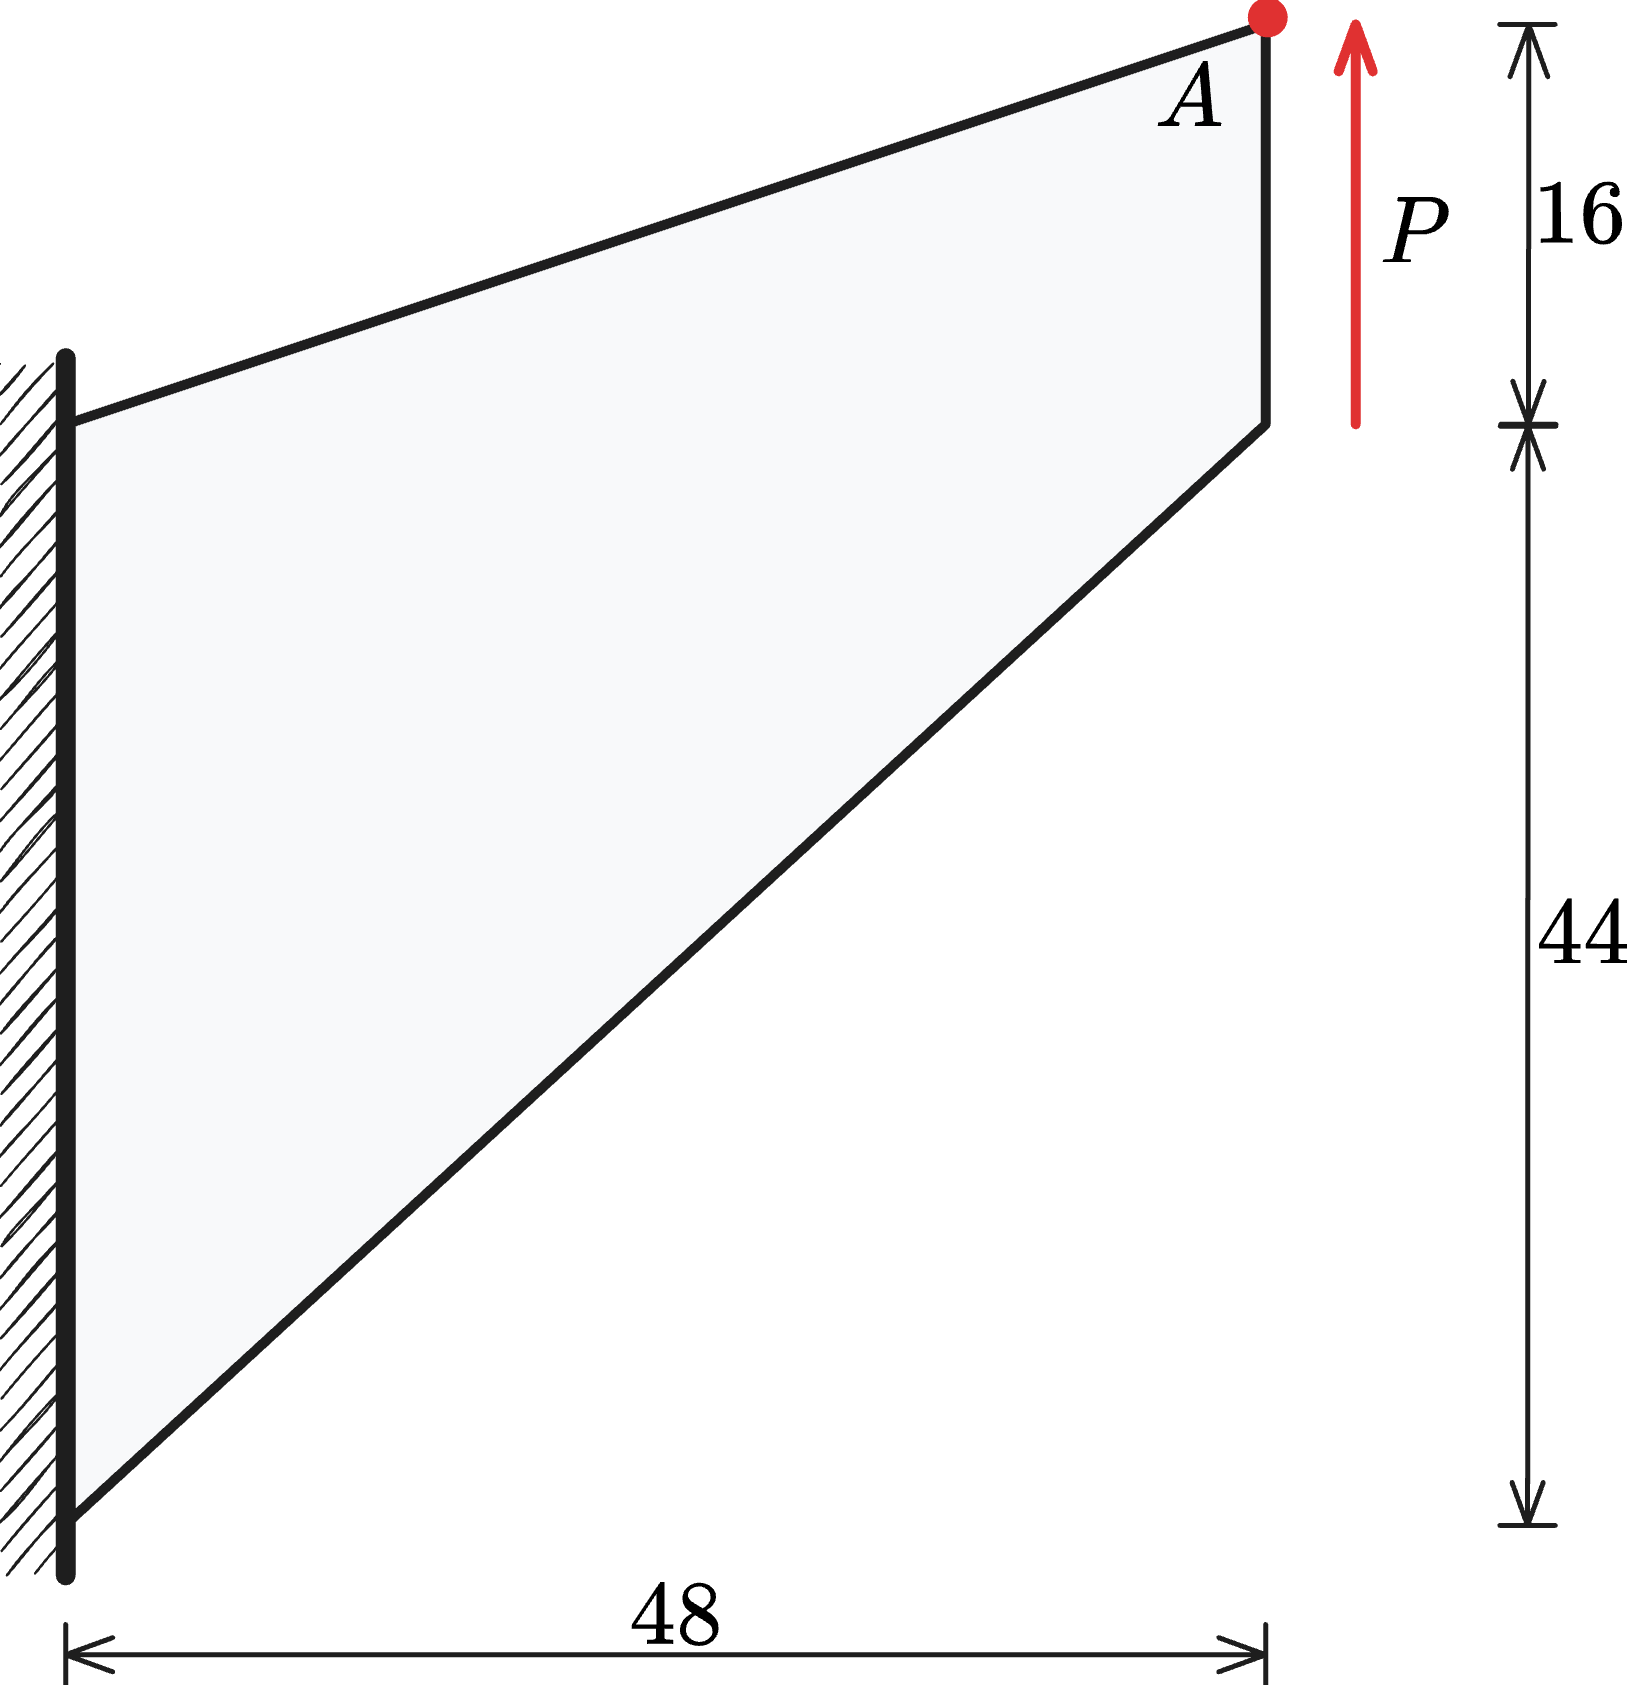
\includegraphics[width=0.5\textwidth]{png/cook_membrane_model.png}
\caption{Illustration of cook membrane problem}\label{fg:cook_illsutration}
\end{figure}

In this test, we focus on the pressure stability of 2D mixed FE--meshfree formulations,
the Figures \ref{fg:cook_membrane_contour_tri3}--\ref{fg:cook_membrane_contour_quad8} show the pressure contour plots for non--uniform Tri3--RK, Tri6--RK, Quad4--RK and Quad8--RK formulations with $r=n_d$ and $r=r_{opt}$, respectively.
The reprocuing kernel meshfree approxiamtions are employed for pressure discretization with characterized support sizes of 1.5 for linear basis function and 2.5 for quadratic basis function.
The results imply that the pressure contour plots with the optimal constraint ratio $r=r_{opt}$ show a more stable and smooth pressure distribution compared to those with the traditional constraint ratio $r=n_d$.

\begin{figure}[H]
\centering
\begin{tabular}{c@{\hspace{5pt}}c@{\hspace{5pt}}c@{\hspace{5pt}}c}
    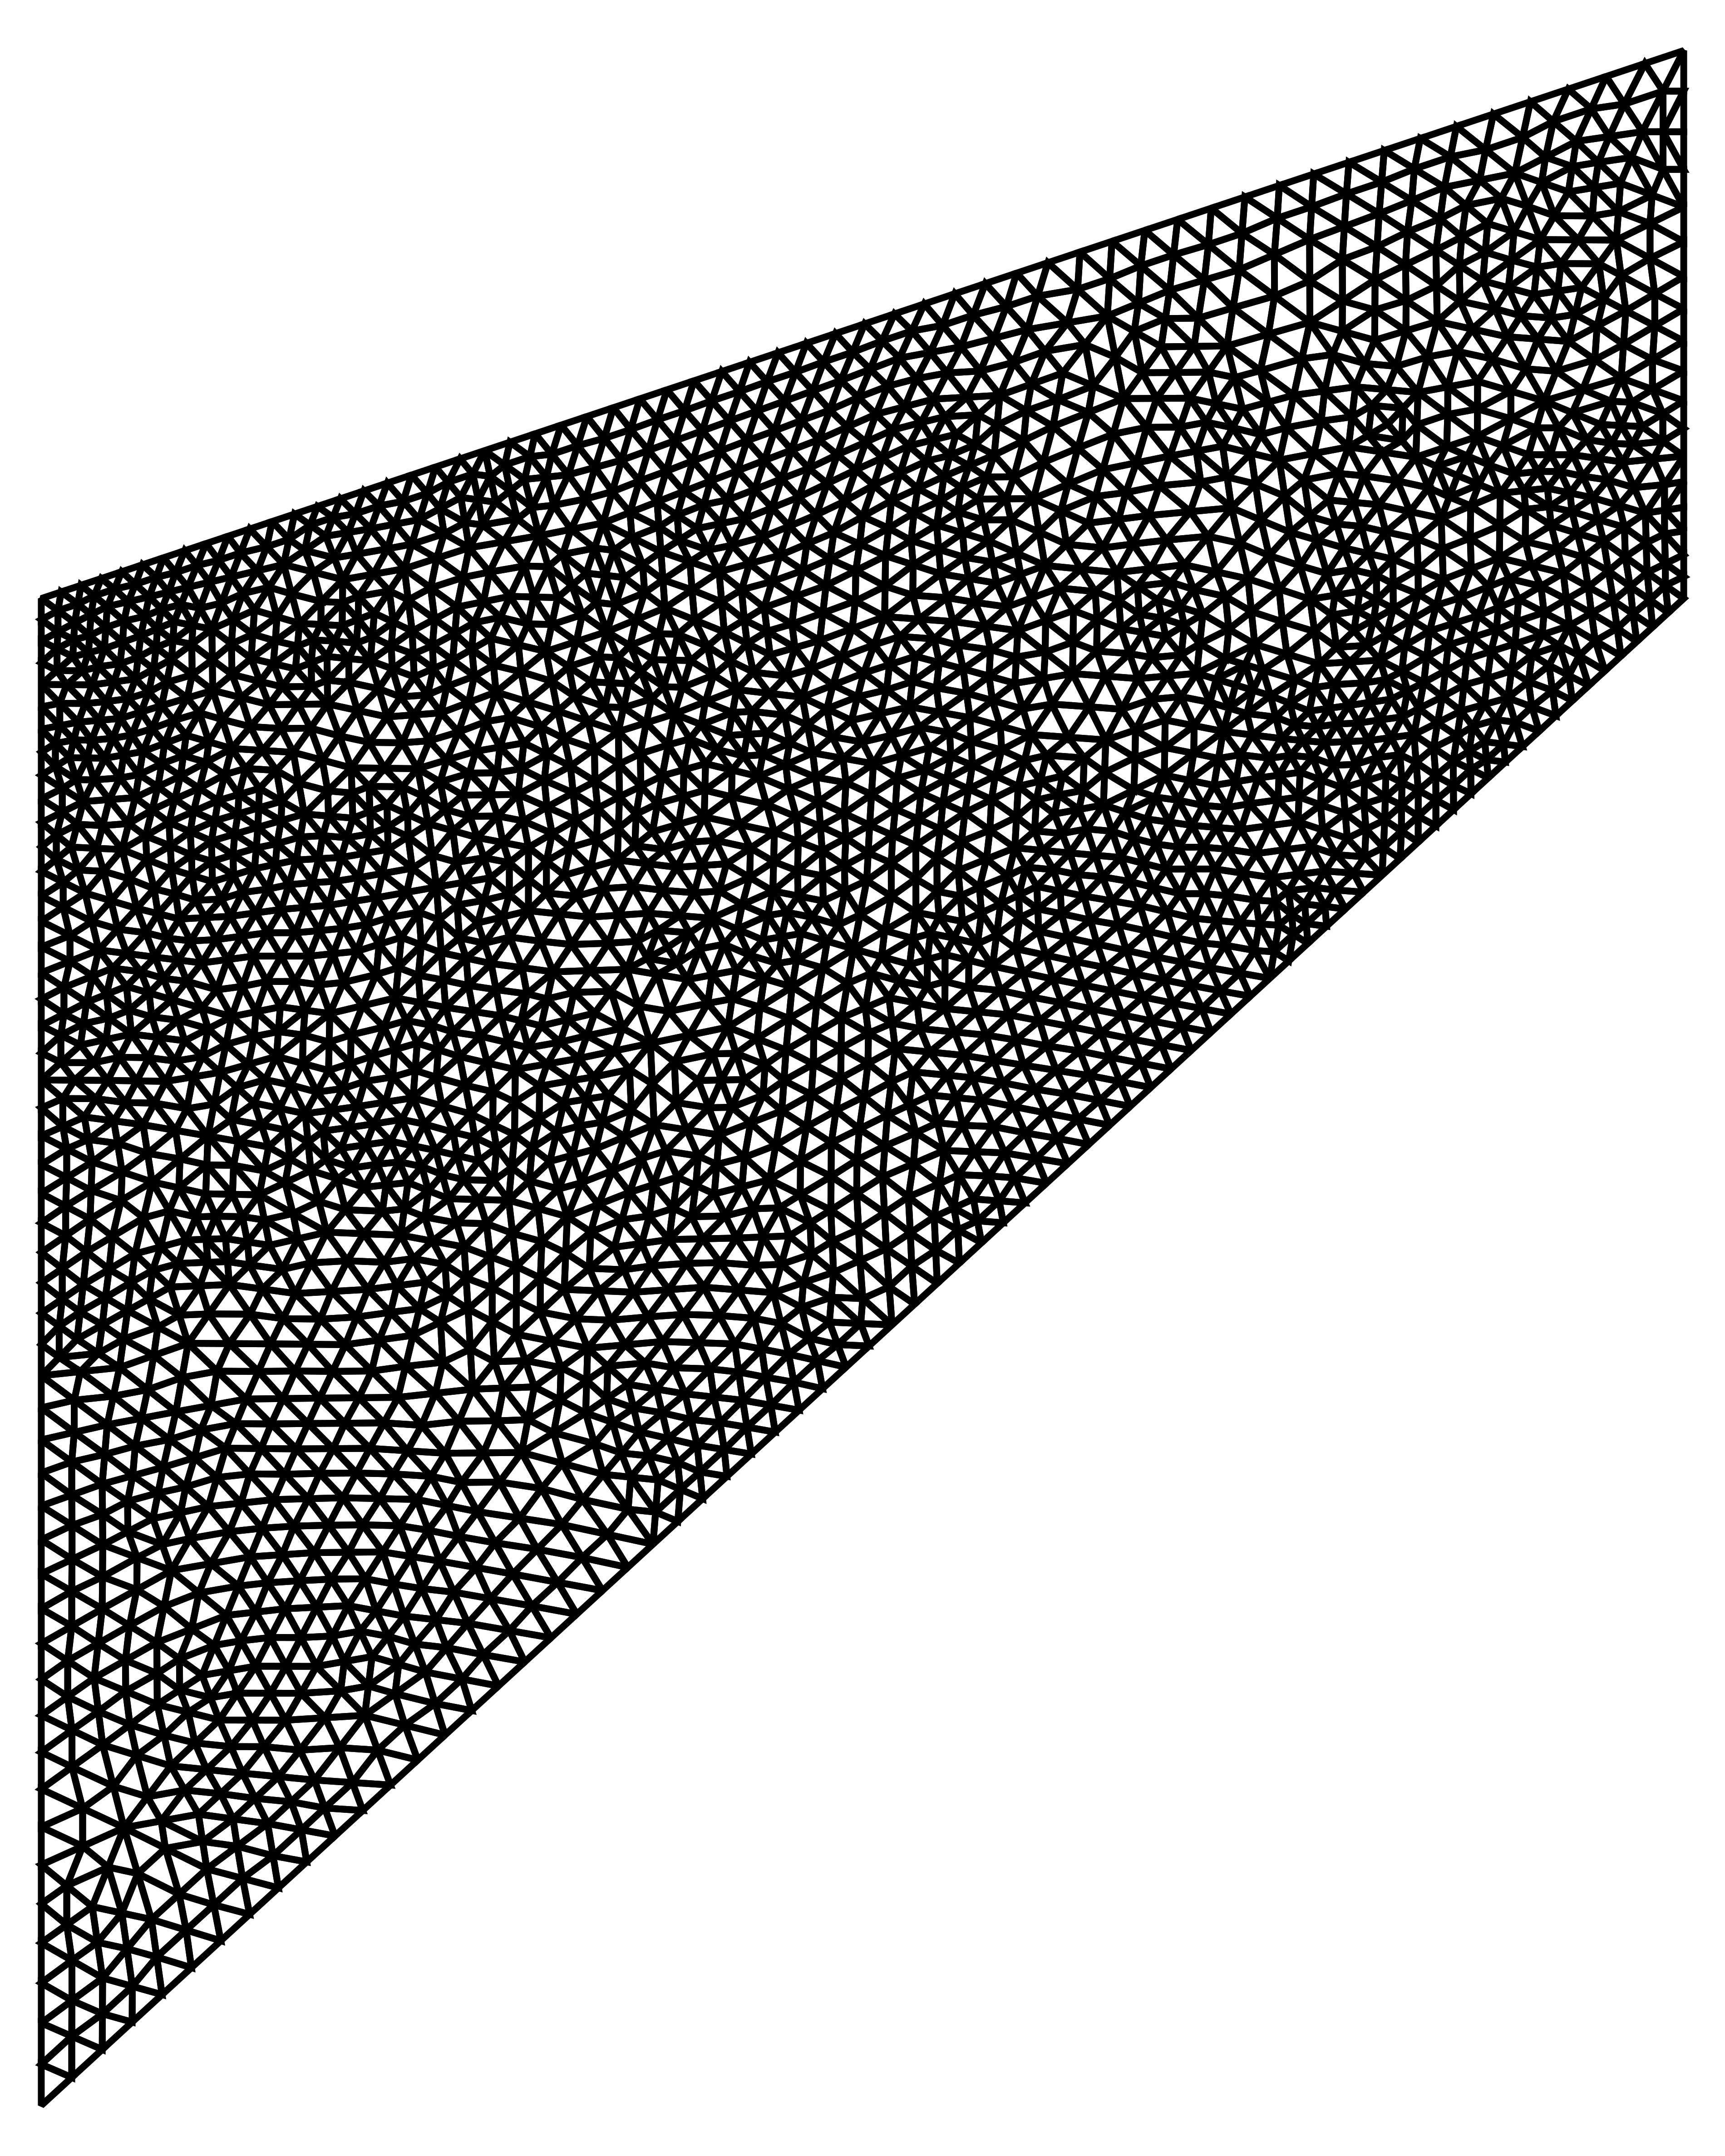
\includegraphics[width=0.33\textwidth]{png/cook_mix_tri3_mesh_2529.png}
    & 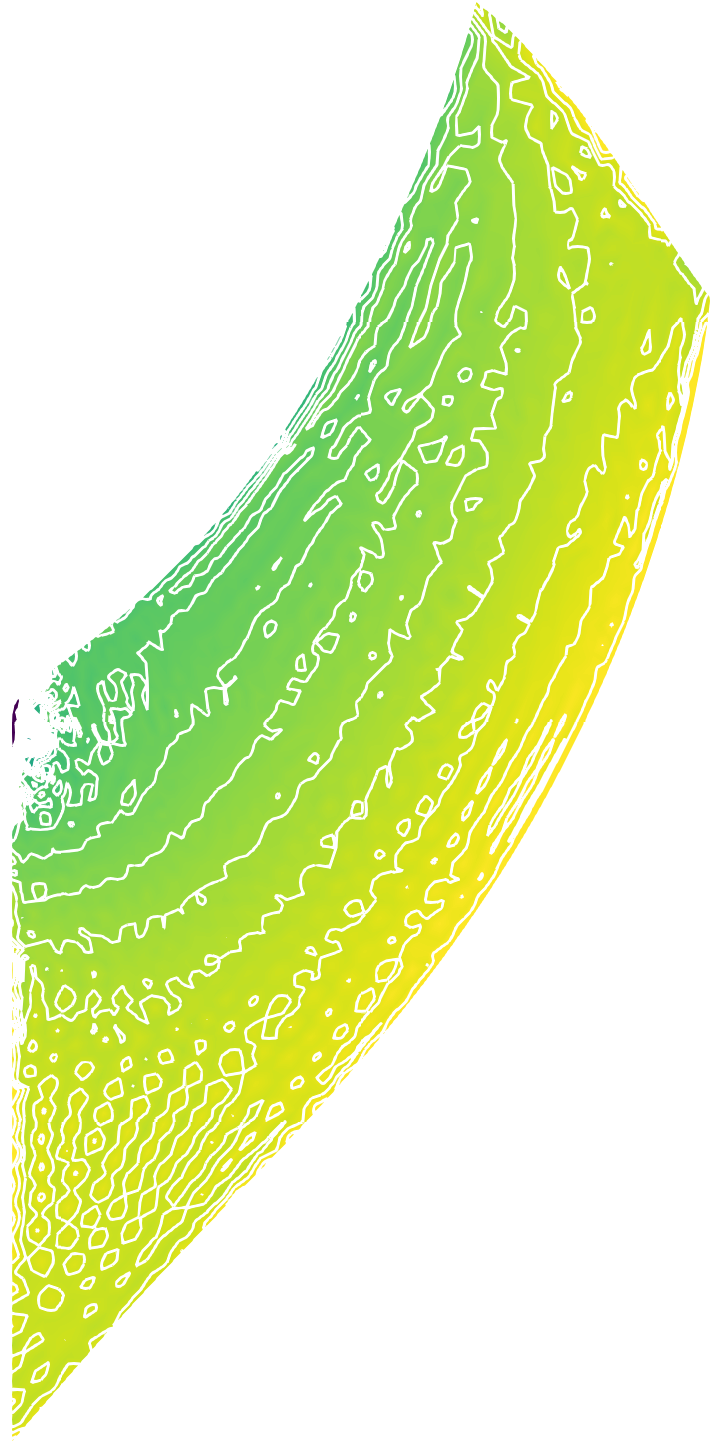
\includegraphics[width=0.28\textwidth]{png/cook_tri3_2529_2529.png}
    & 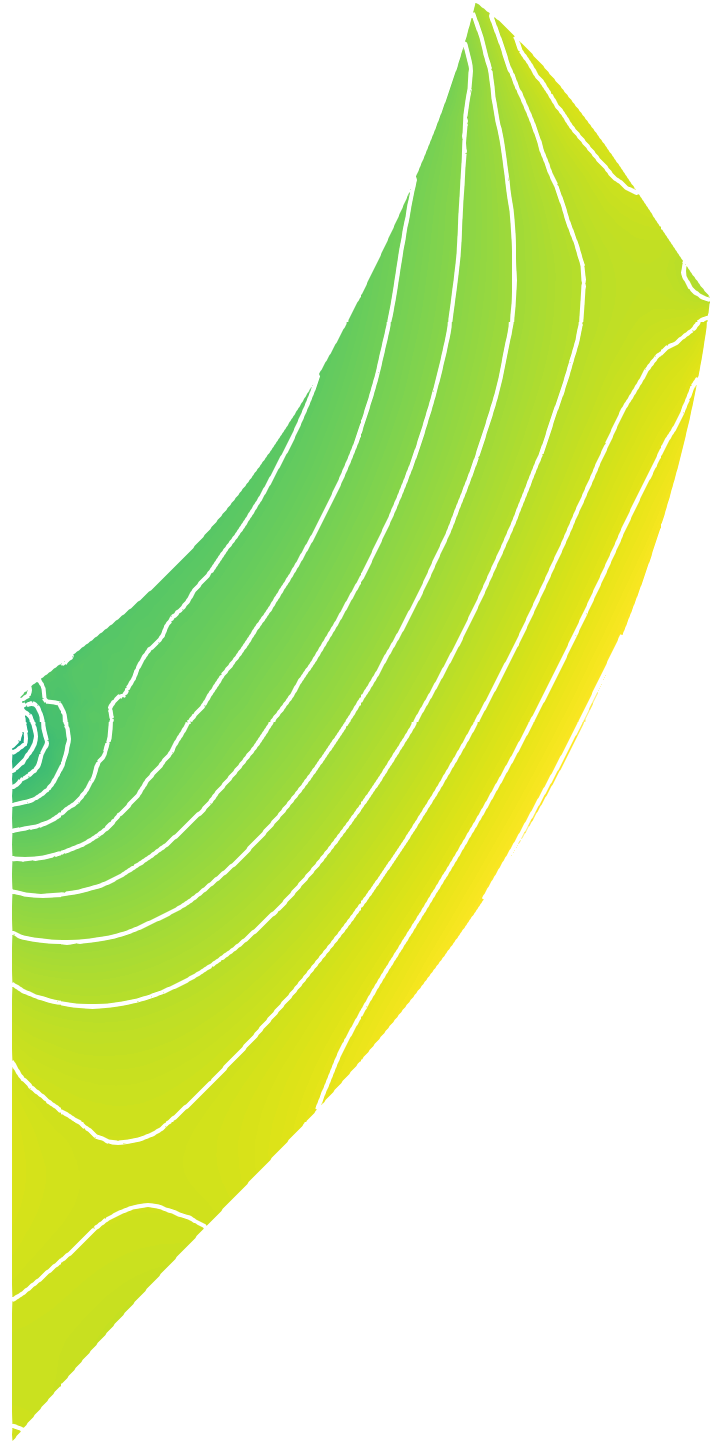
\includegraphics[width=0.28\textwidth]{png/cook_tri3_2529_658.png}
    & 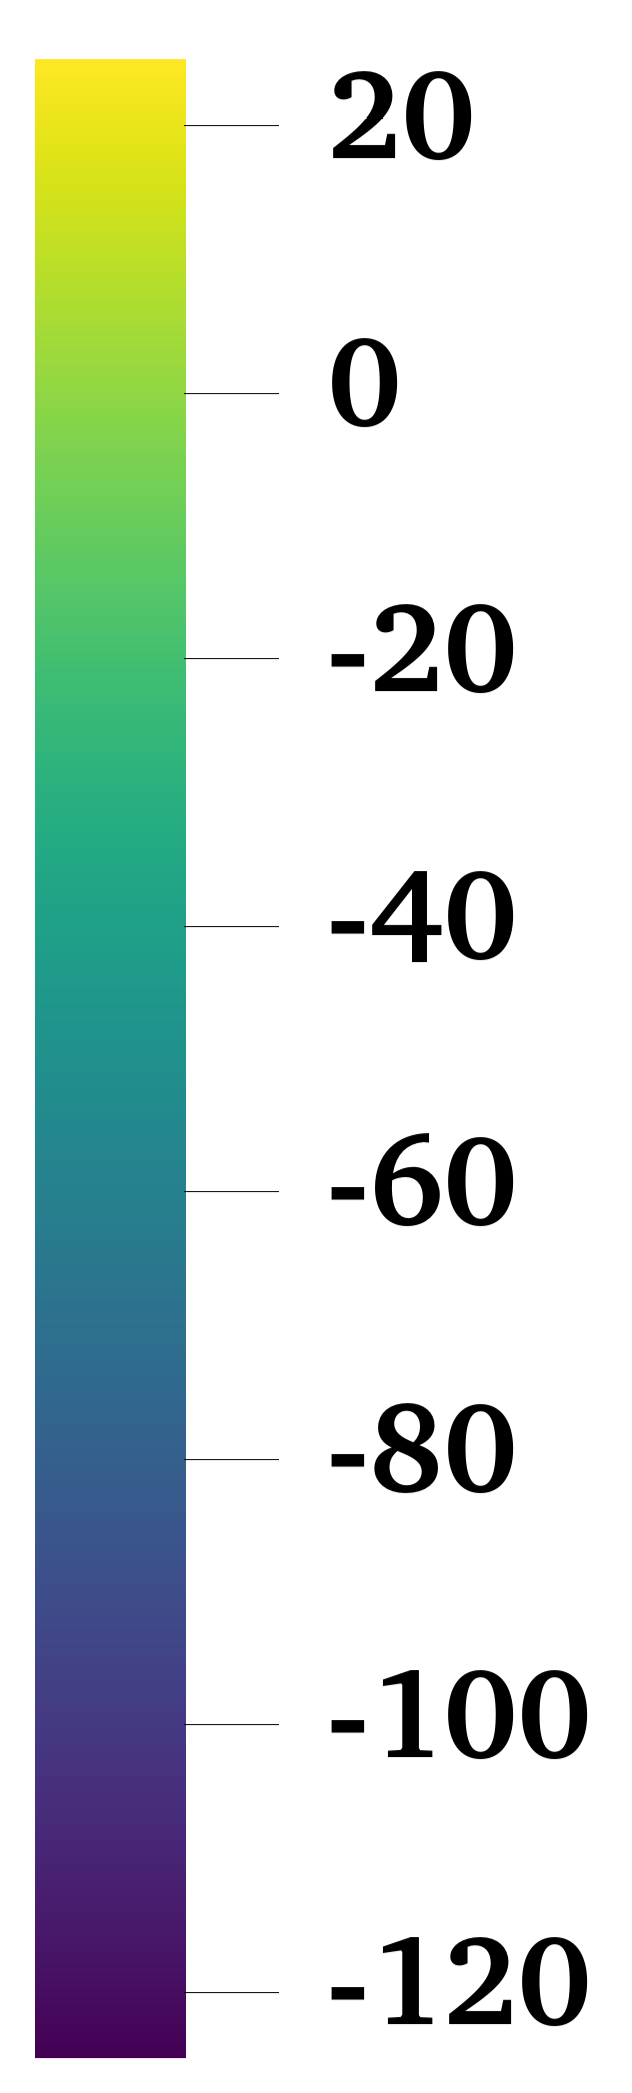
\includegraphics[width=0.1\textwidth]{png/legend.png}
    \\
    $n_u = 2529$ & $r = n_d$ & $r = r_{opt}$ &
\end{tabular}
\caption{Comparison of pressure contour plots for cook membrane problem with Tri3--RK}\label{fg:cook_membrane_contour_tri3}
\end{figure}

\begin{figure}[H]
\centering
\begin{tabular}{c@{\hspace{5pt}}c@{\hspace{5pt}}c@{\hspace{5pt}}c}
    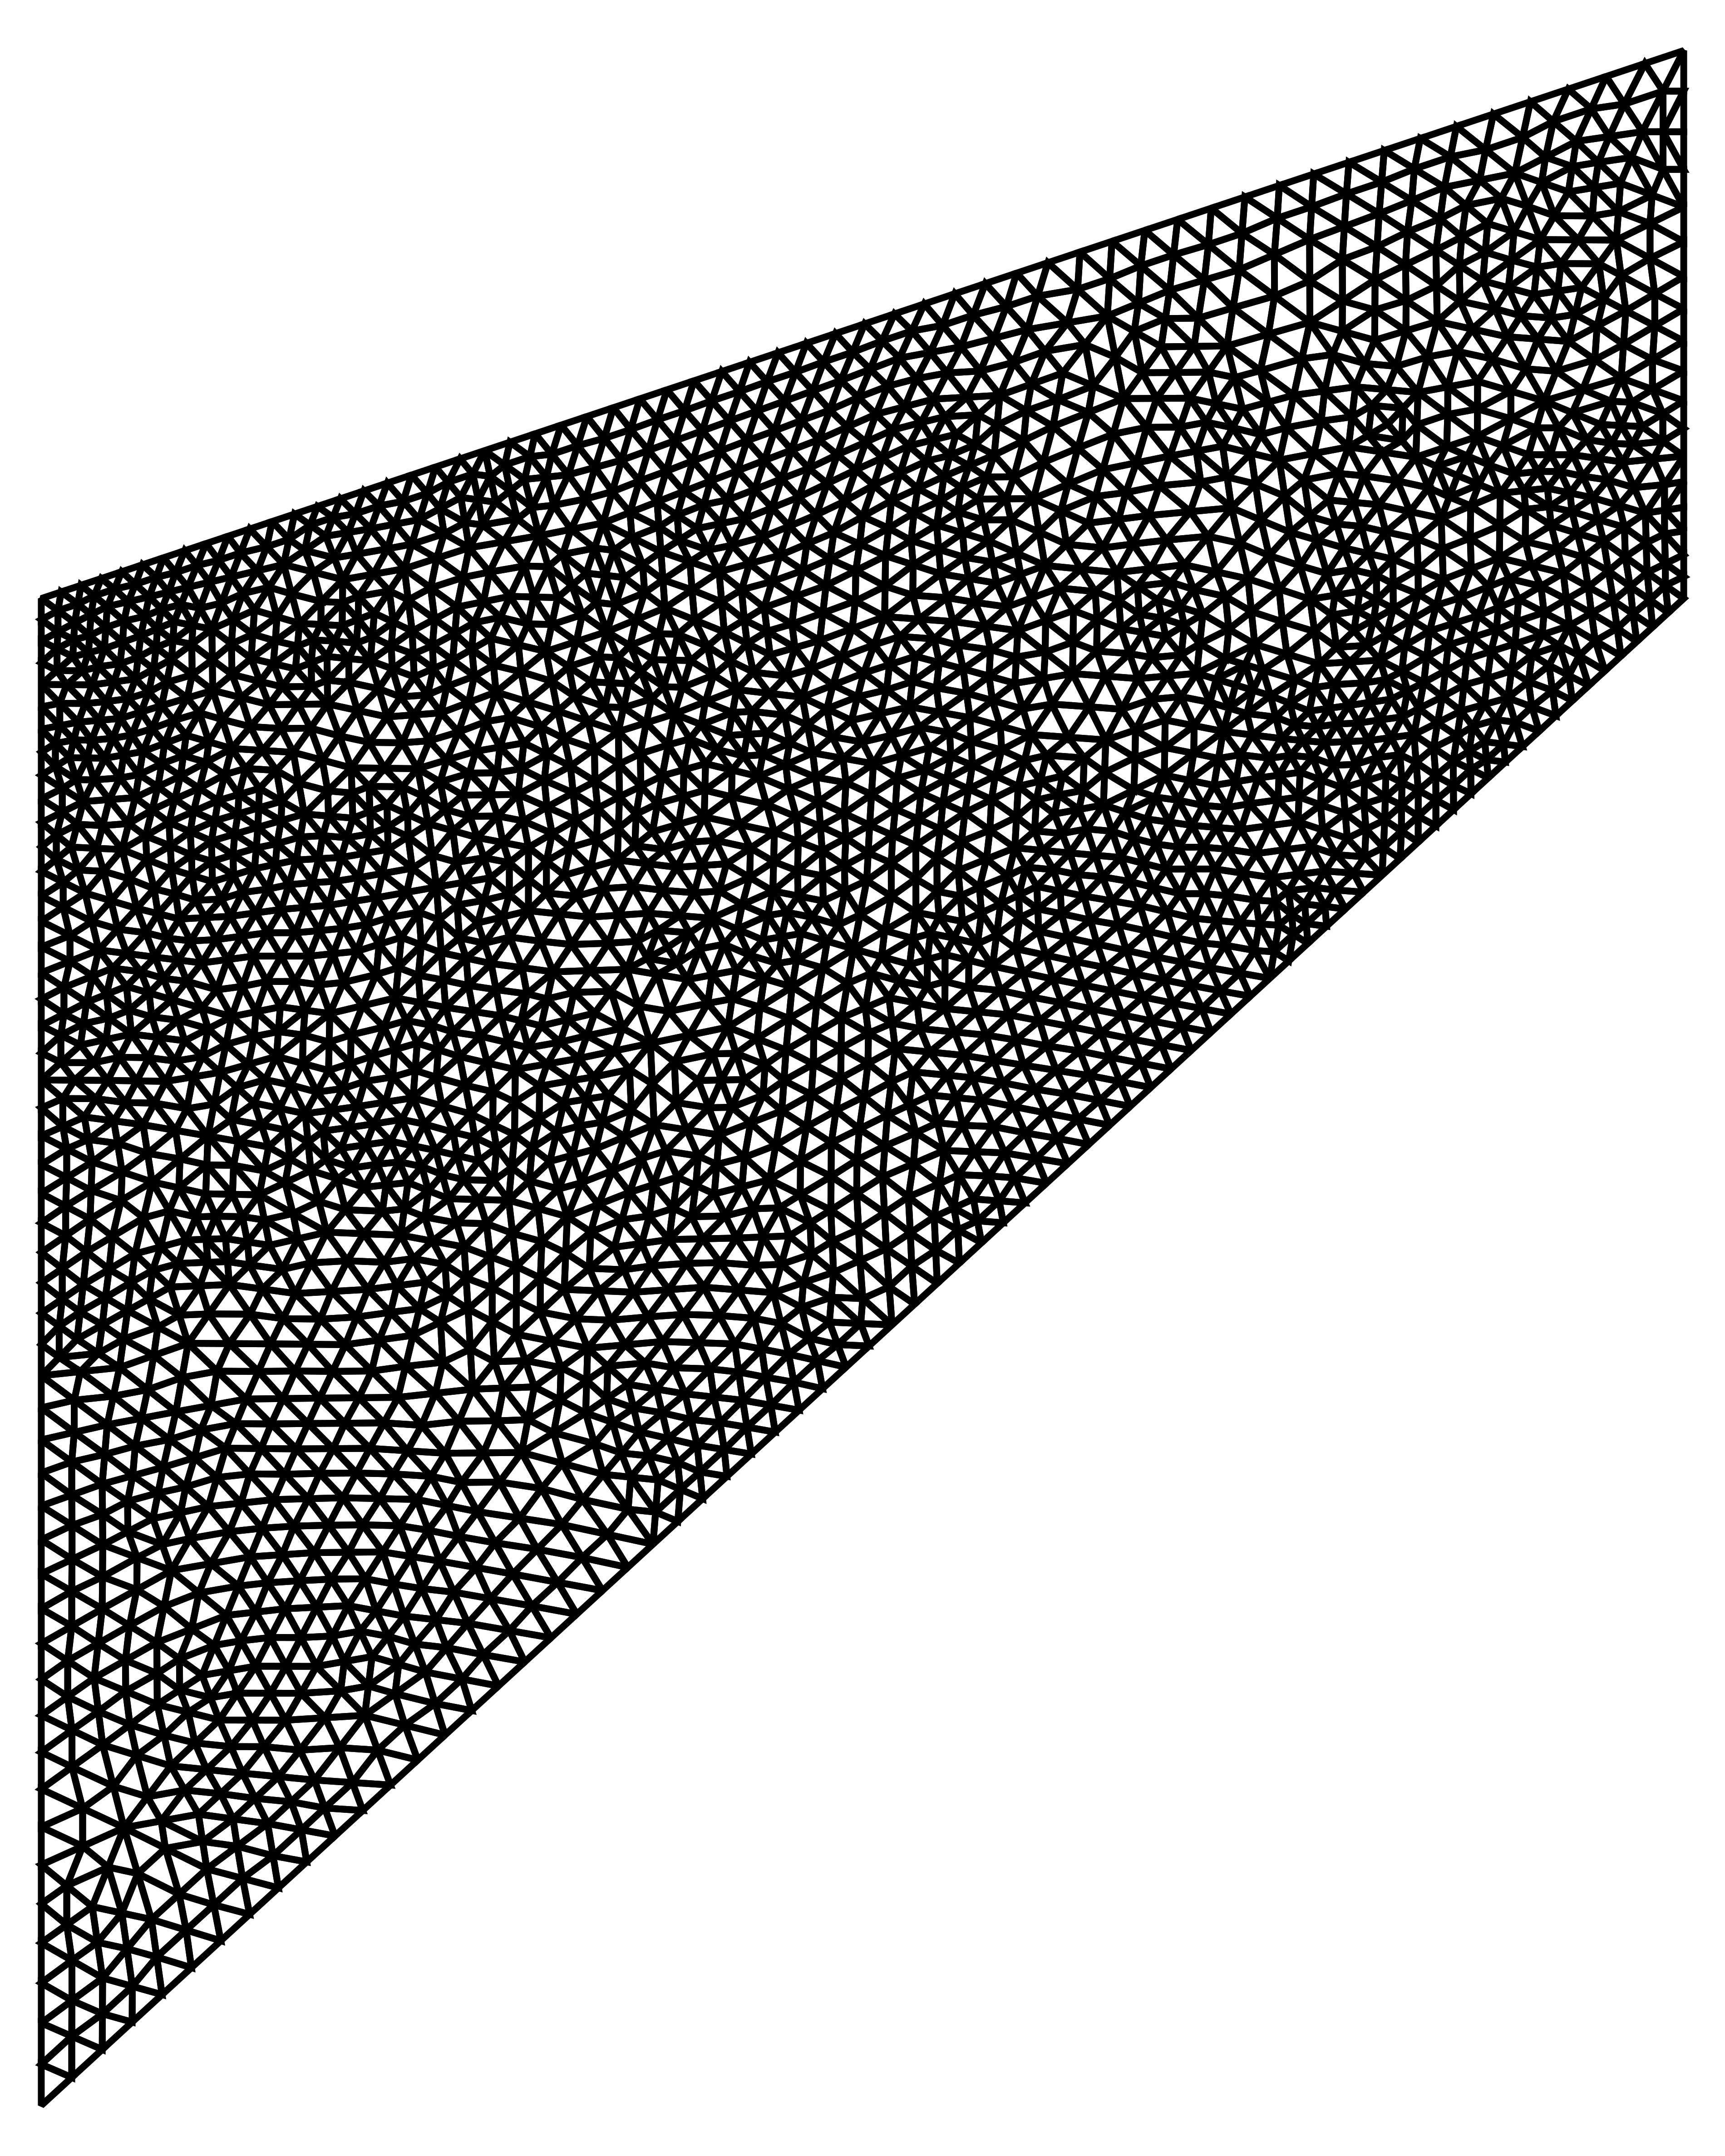
\includegraphics[width=0.33\textwidth]{png/cook_mix_tri3_mesh_2529.png}
    & 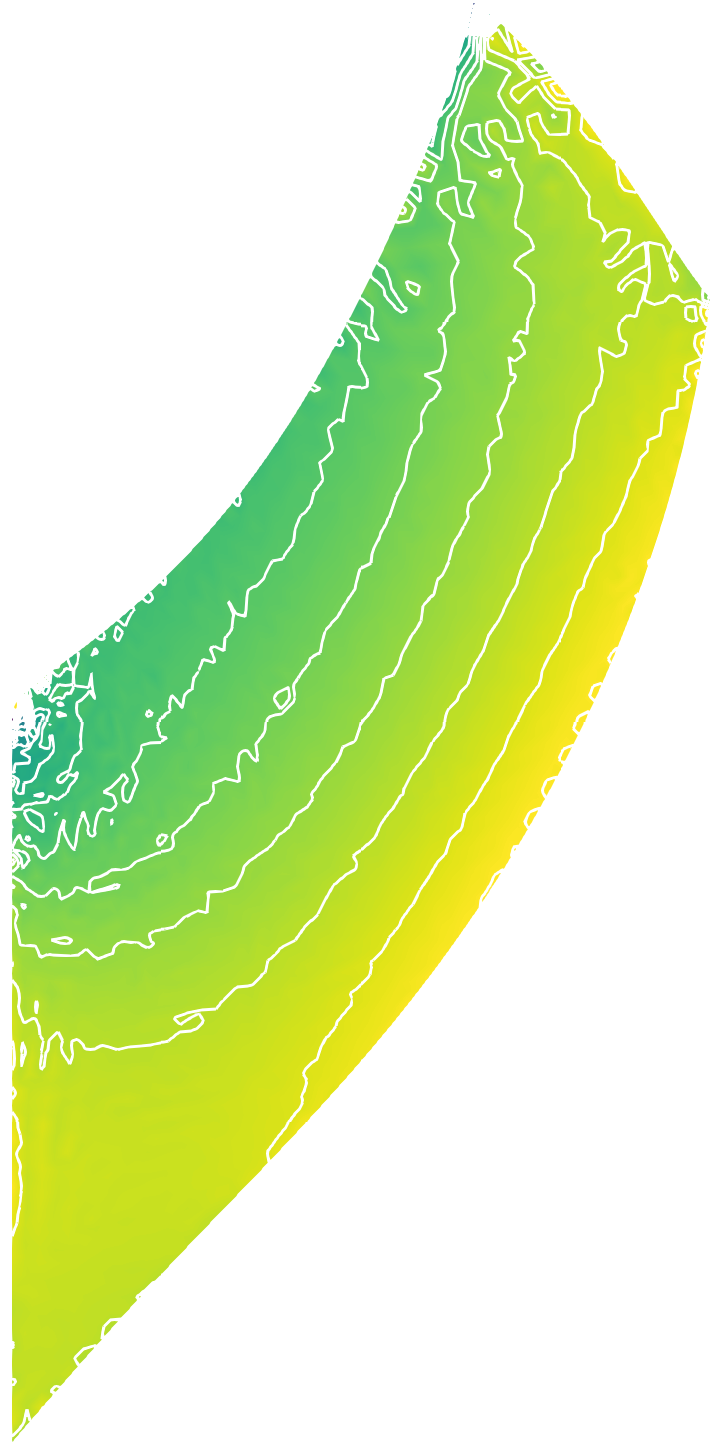
\includegraphics[width=0.28\textwidth]{png/cook_tri6_2529_2529.png}
    & 
\includegraphics[width=0.28\textwidth]{png/cook_tri6_2529_658.png}
    & 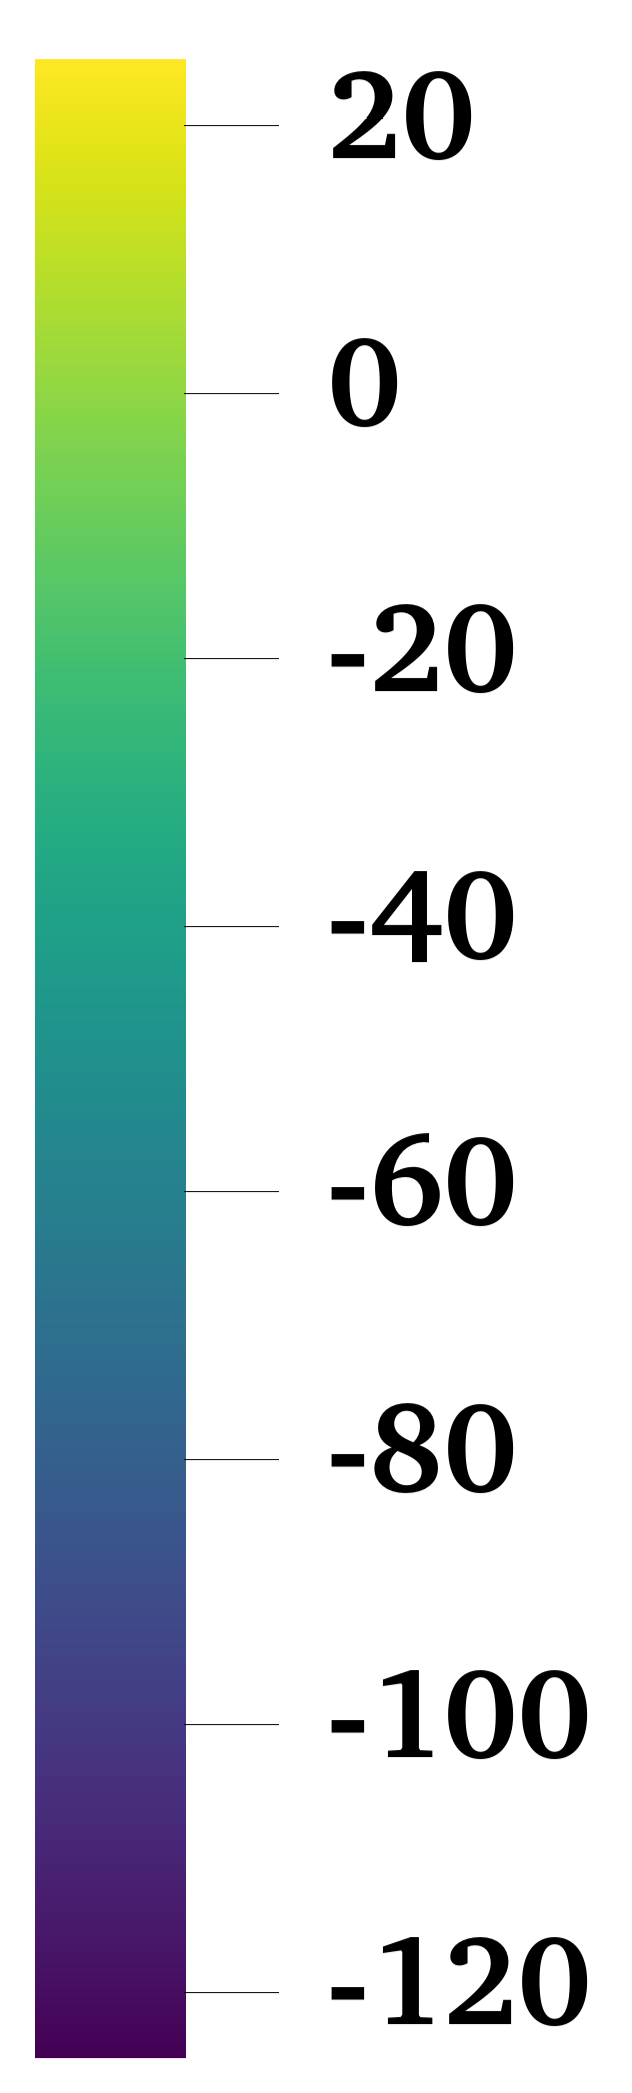
\includegraphics[width=0.1\textwidth]{png/legend.png}
    \\
    $n_u = 2529$ & $r = n_d$ & $r = r_{opt}$ &
\end{tabular}
\caption{Comparison of pressure contour plots for cook membrane problem with Tri6--RK}\label{fg:cook_membrane_contour_tri6}
\end{figure}

\begin{figure}[H]
\centering
\begin{tabular}{c@{\hspace{5pt}}c@{\hspace{5pt}}c@{\hspace{5pt}}c}
    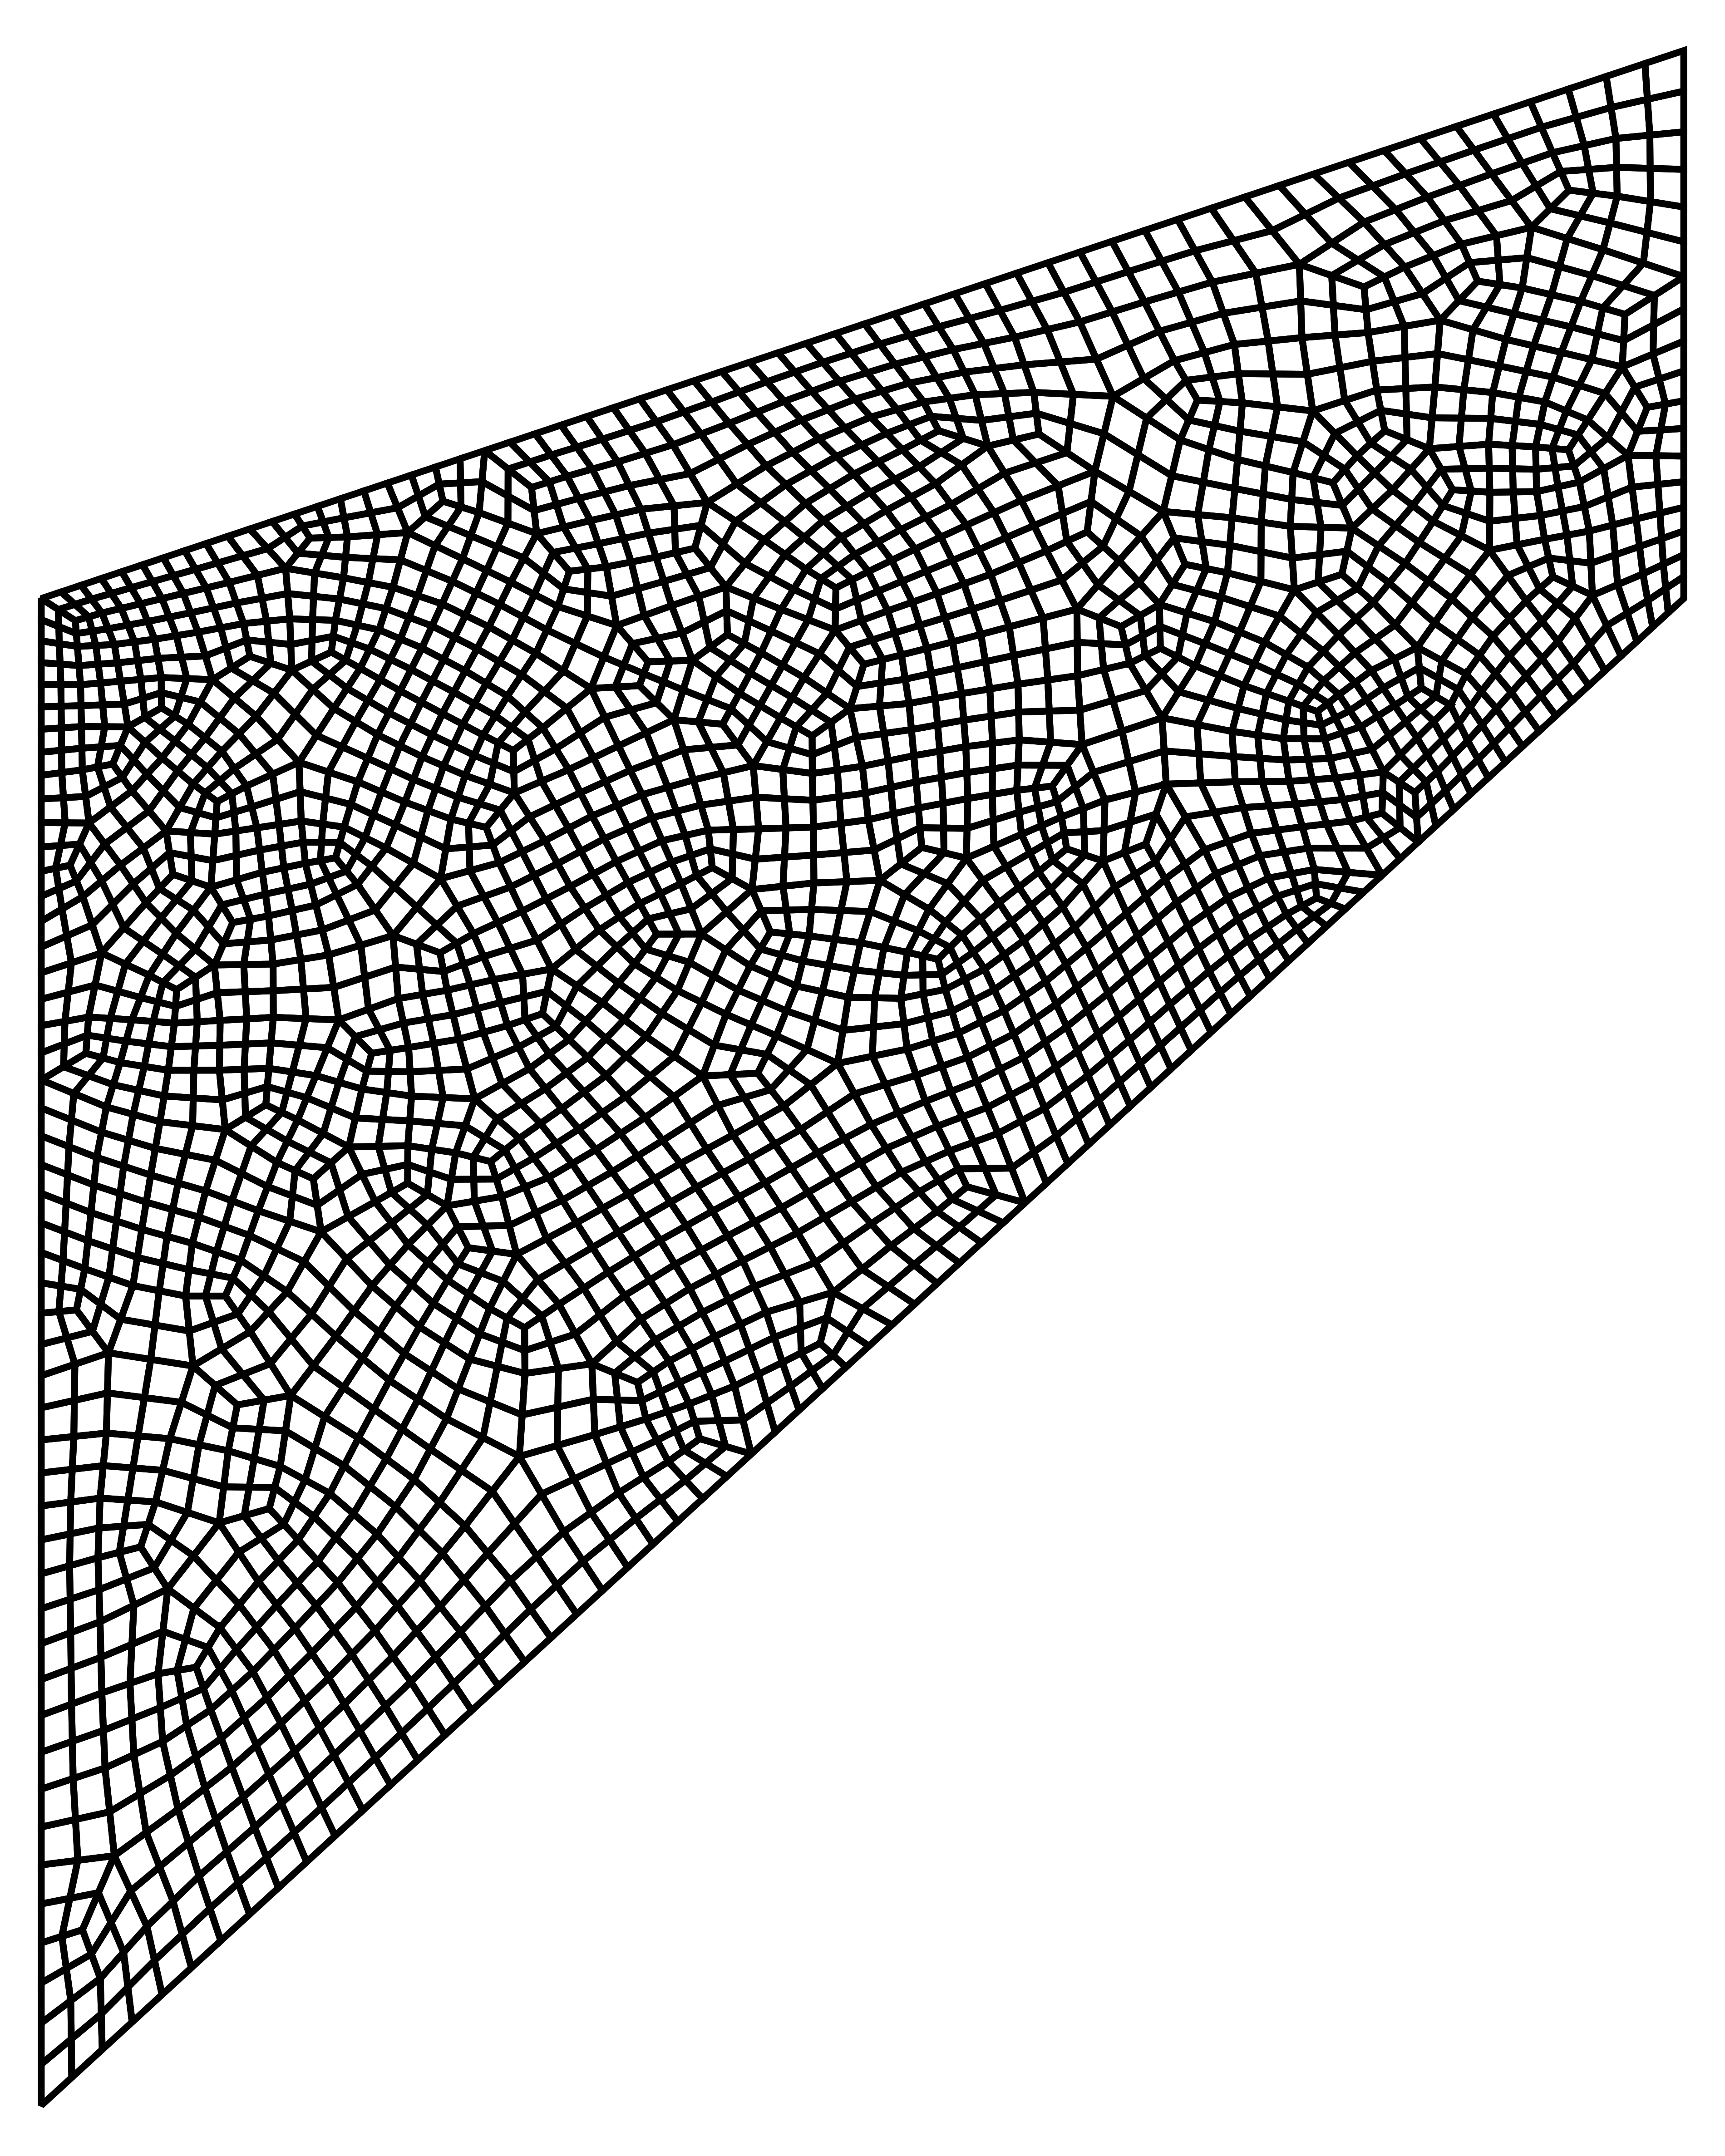
\includegraphics[width=0.33\textwidth]{png/cook_mix_quad_mesh_2485.png}
    & 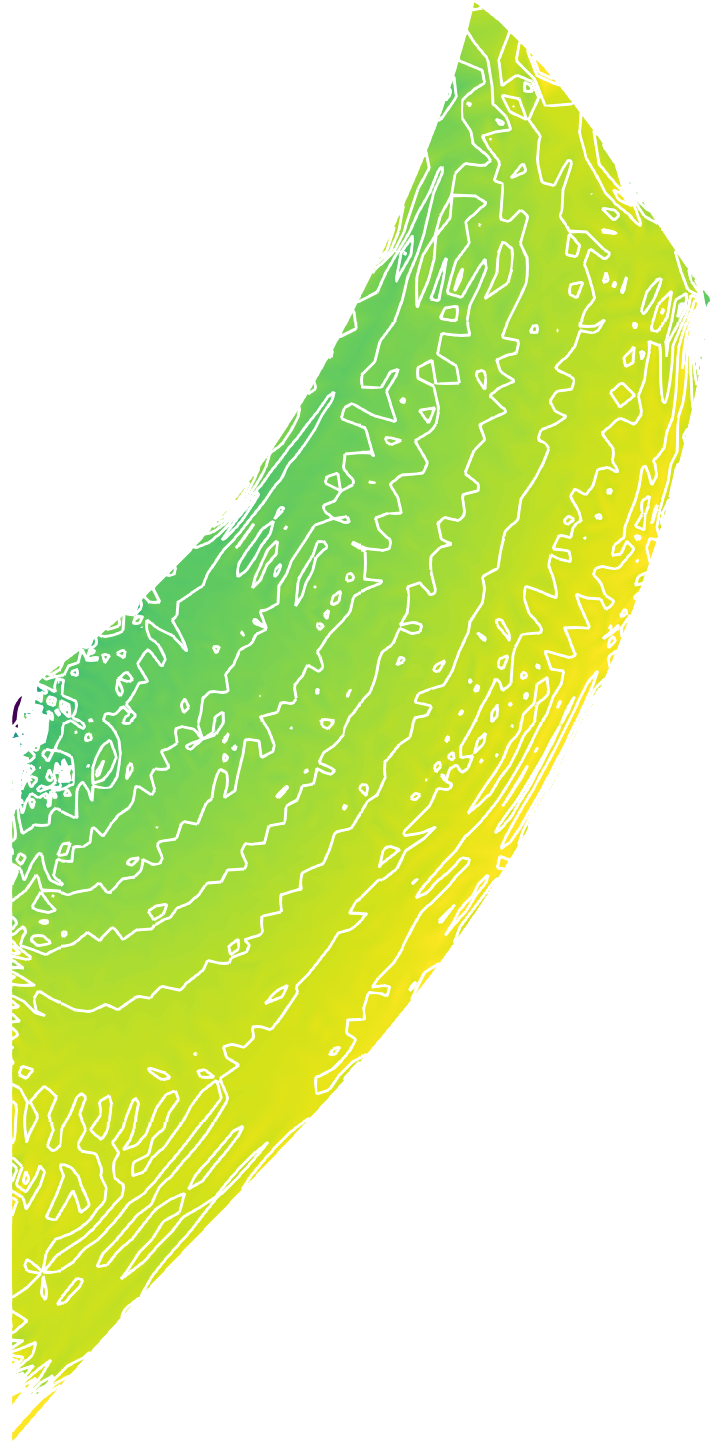
\includegraphics[width=0.28\textwidth]{png/cook_quad4_2485_2485.png}
    & 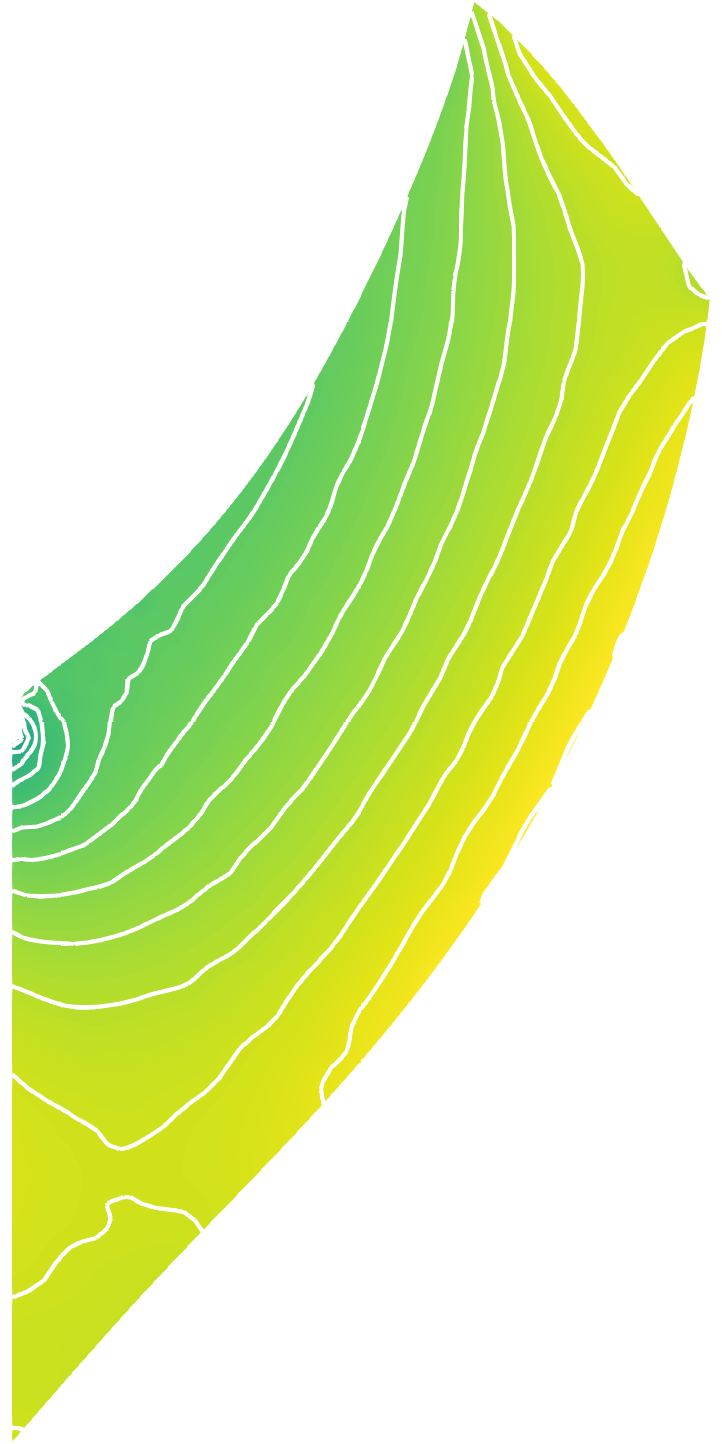
\includegraphics[width=0.28\textwidth]{png/cook_quad4_2485_647.png}
    & 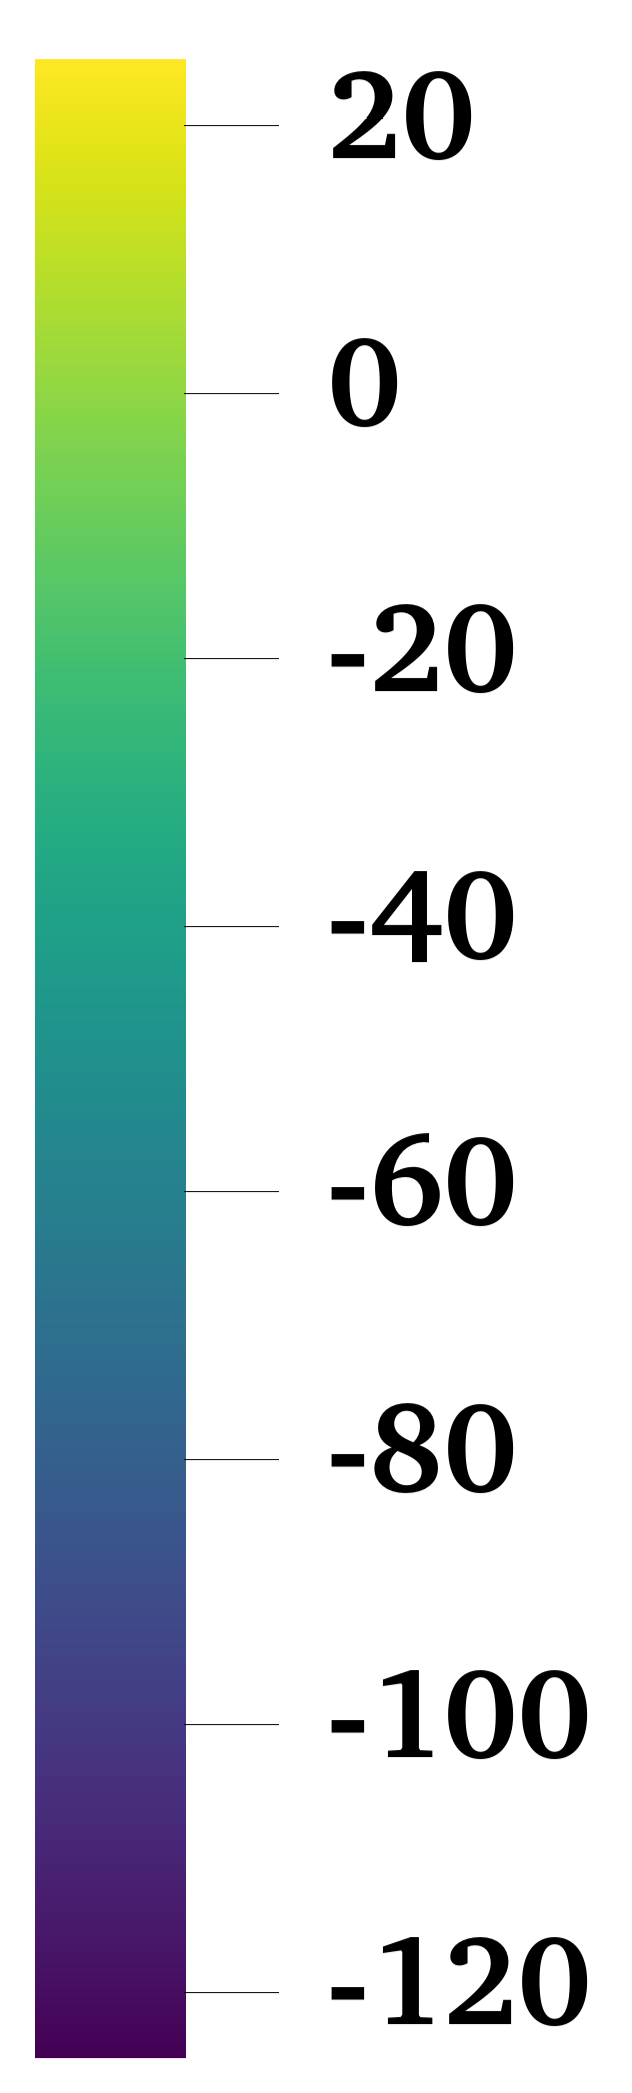
\includegraphics[width=0.1\textwidth]{png/legend.png}
    \\
    $n_u = 2485$ & $r = n_d$ & $r = r_{opt}$ &
\end{tabular}
\caption{Comparison of pressure contour plots for cook membrane problem with Quad4--RK}\label{fg:cook_membrane_contour_quad4}
\end{figure}

\begin{figure}[H]
\centering
\begin{tabular}{c@{\hspace{5pt}}c@{\hspace{5pt}}c@{\hspace{5pt}}c}
    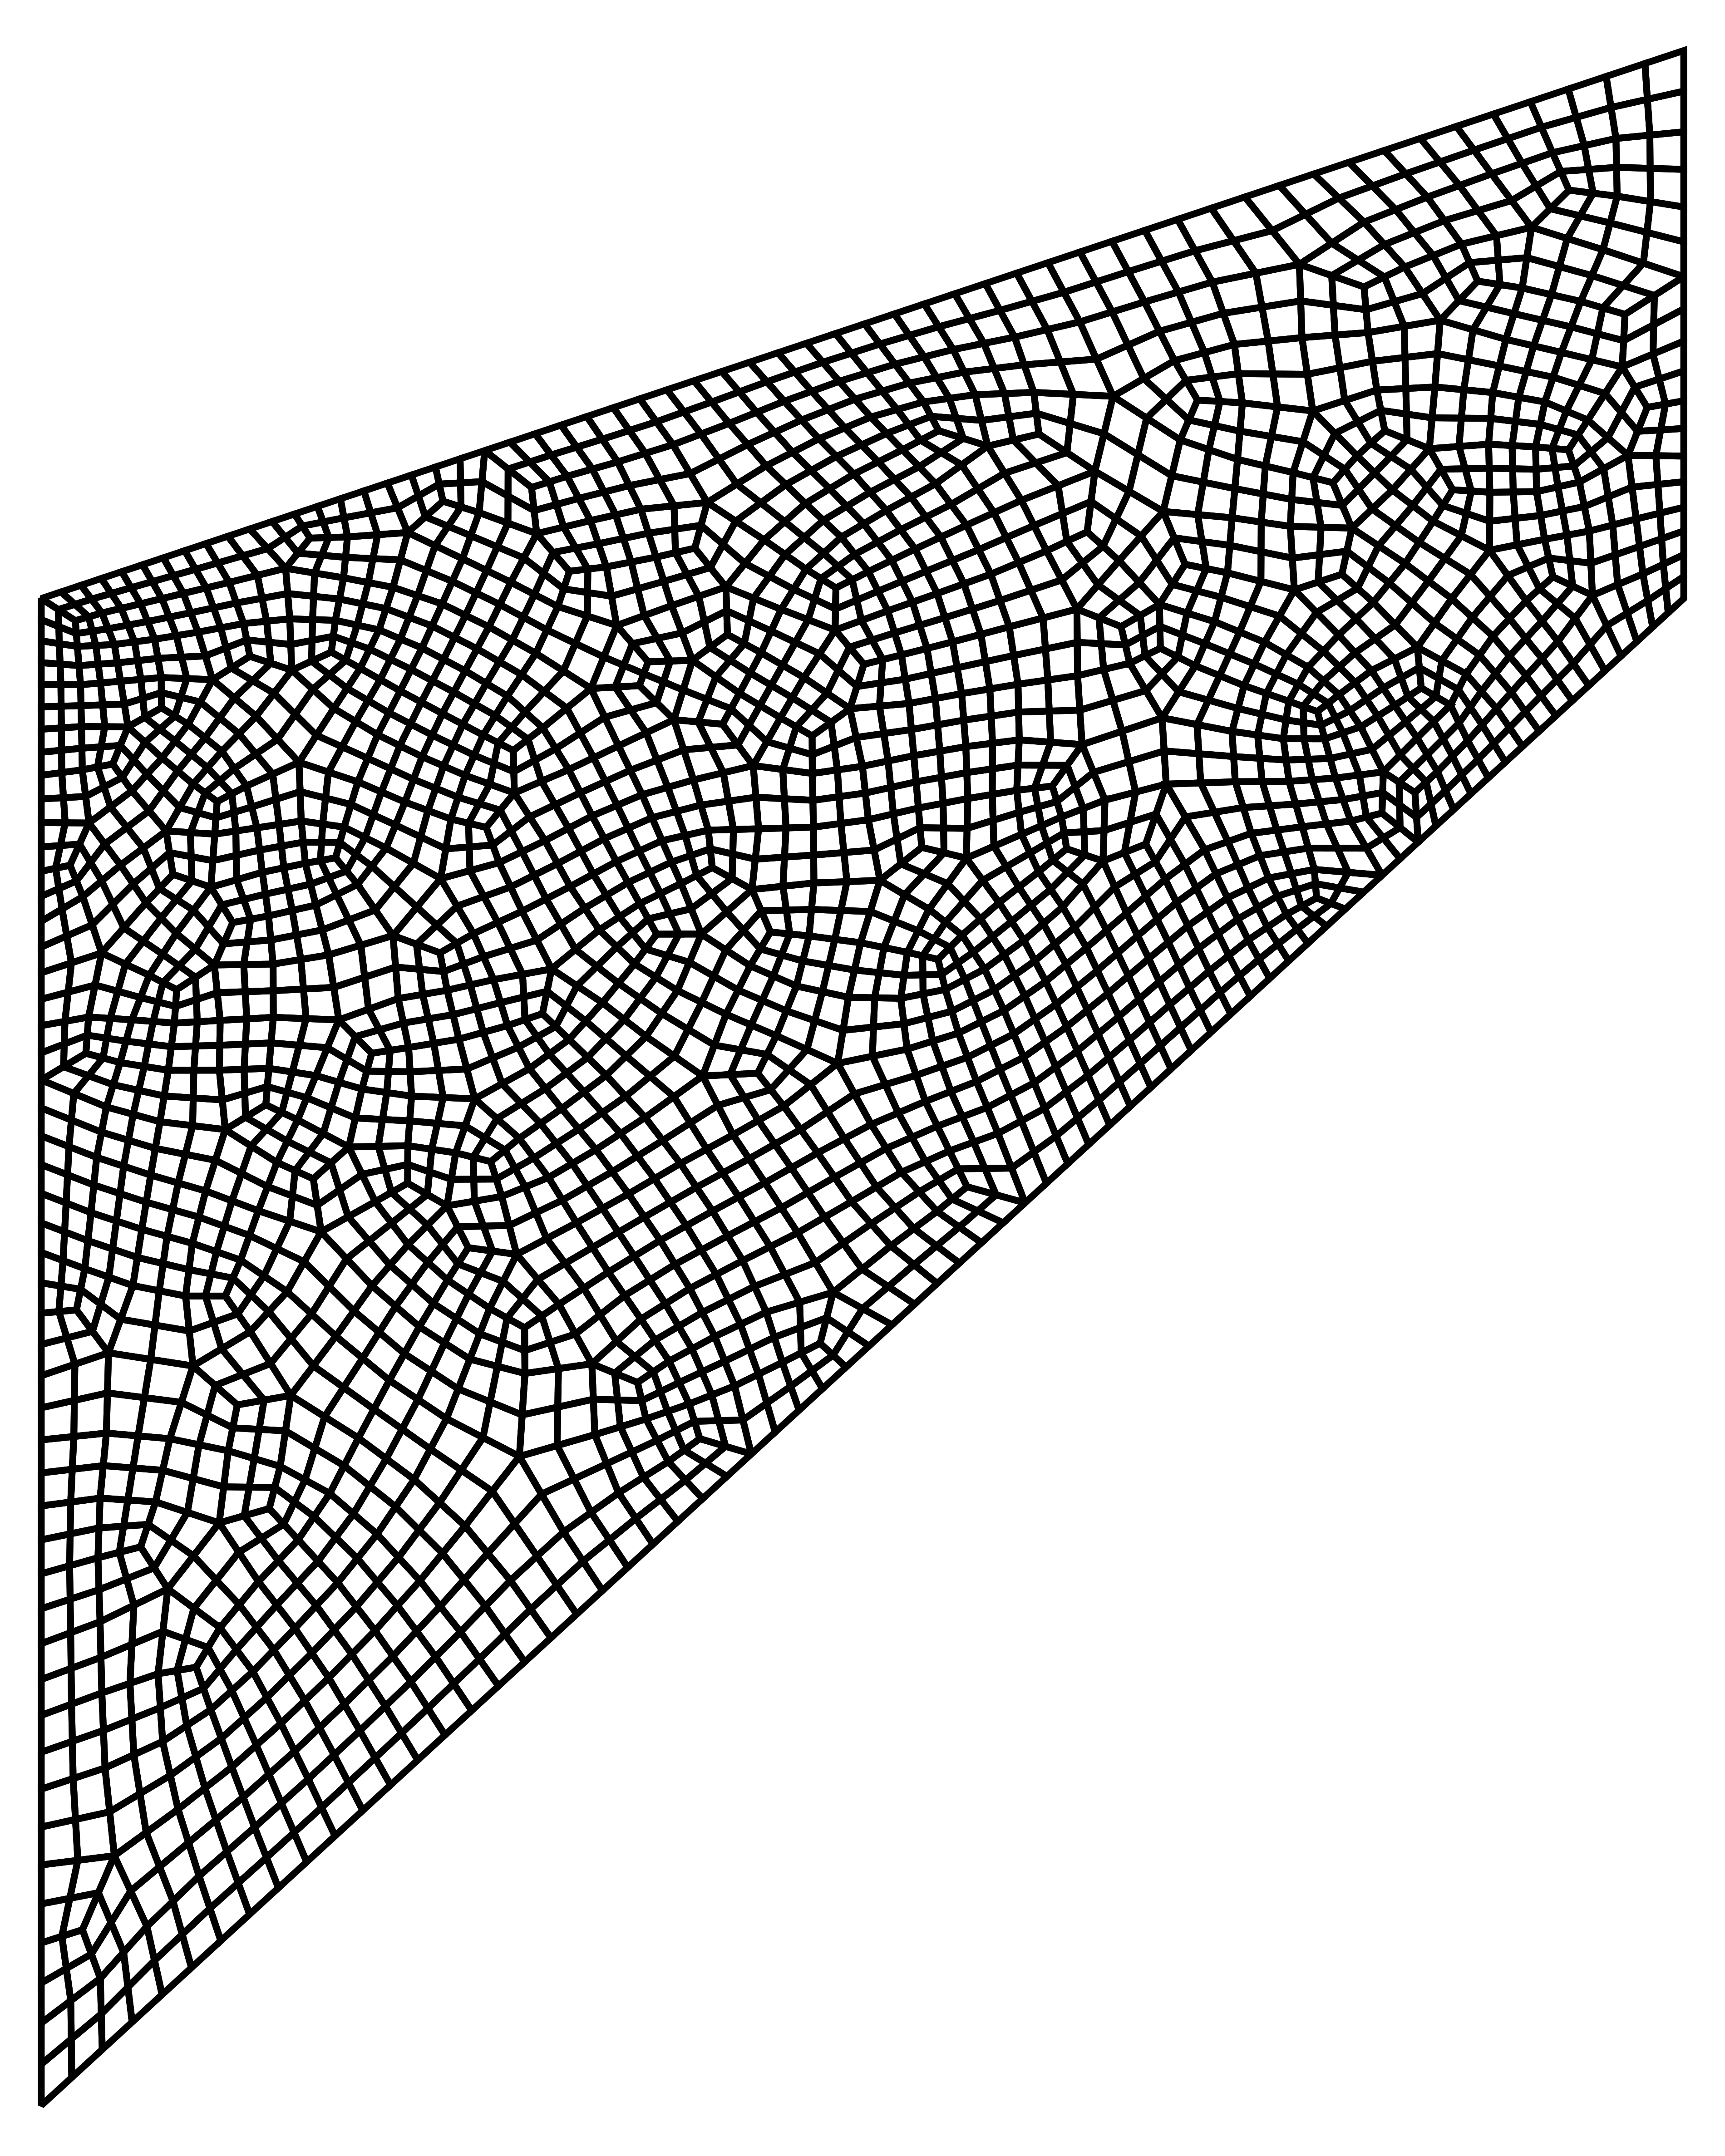
\includegraphics[width=0.33\textwidth]{png/cook_mix_quad_mesh_2485.png}
    & 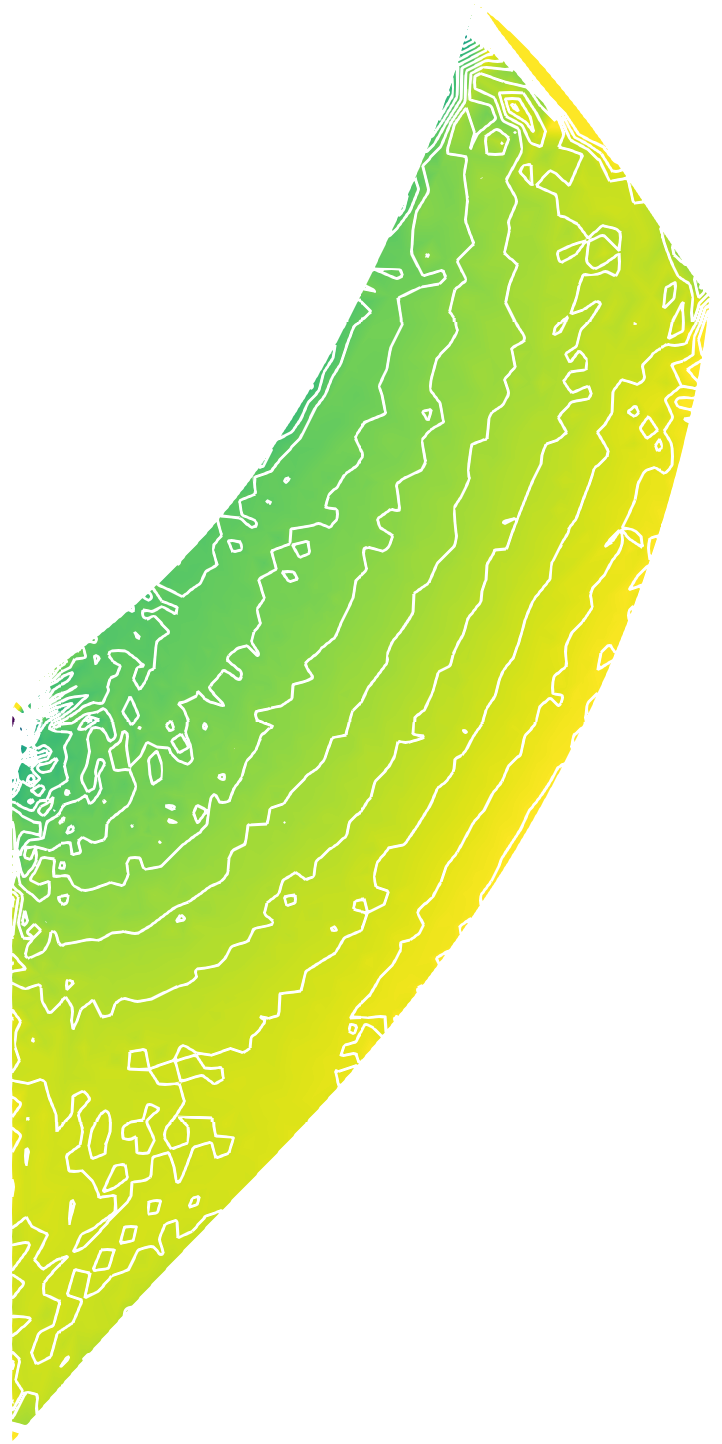
\includegraphics[width=0.28\textwidth]{png/cook_quad8_1889_1889.png}
    & 
\includegraphics[width=0.28\textwidth]{png/cook_quad8_1889_647.png}
    & 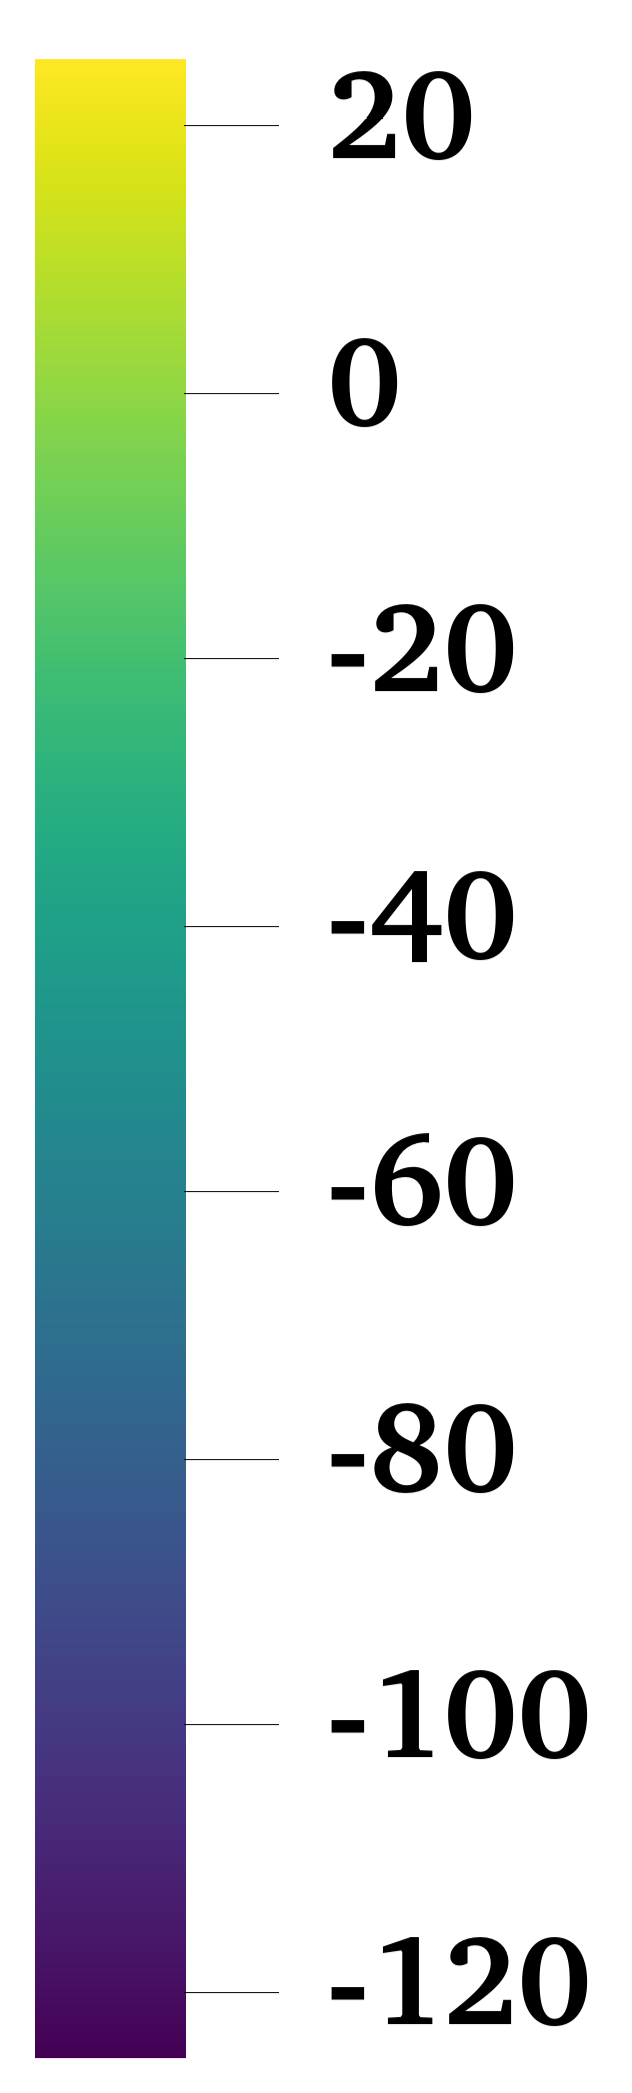
\includegraphics[width=0.1\textwidth]{png/legend.png}
    \\
    $n_u = 1889$ & $r = n_d$ & $r = r_{opt}$ &
\end{tabular}
\caption{Comparison of pressure contour plots for cook membrane problem with Quad8--RK}\label{fg:cook_membrane_contour_quad8}
\end{figure}
